\documentclass[12pt]{article}
\usepackage[utf8]{inputenc}
\usepackage[T1]{fontenc}
\usepackage[french]{babel}
\usepackage{graphicx}
\usepackage{hyperref}
\usepackage{geometry}
\usepackage{float}

\geometry{a4paper, margin=1in}

\begin{document}

\begin{titlepage}
    \centering
    
\includegraphics[width=0.4\textwidth]{logo.png}\par\vspace{1cm}
    \vspace{2cm}
    {\huge\bfseries Compte Rendu IoT\par}
    \vspace{0.5cm}
    {\Large\bfseries TP 01: NodeRed, MQTT, NodemCU\par}
    \vspace{2.5cm}
    {\large
    \begin{tabular}{rl}
      \textbf{Module:} & Internet des Objets (IoT) \\[0.8em]
      \textbf{Niveau:}  & IAGI - 2\textsuperscript{ème} année \\[0.8em]
      \textbf{Encadrant:} & Prof. Hain \\[0.8em]
      \textbf{Auteurs:} & Rabya RAGHIB \\
                        & Imane SAOUDI \\
                        & Nouhaila NOKRY \\
                        & Abdellah MOGHANDEZ \\
                        & Mohamed AMANE
    \end{tabular}}
    \vspace{2cm}
    
    \vfill
    {\large Année universitaire 2025/2026\par}
\end{titlepage}

\section*{Atelier 15}

\textbf{Lien Wokwi :} \url{https://wokwi.com/projects/462396191798252545}

\vspace{0.3cm}
\textbf{Description :} Un montage permettant de contrôler à distance une LED connectée à un ESP32. En envoyant des messages (`on`, `off`) via le broker HiveMQ, l'ESP32 lit le topic et met à jour l'état du LED.
\vspace{0.5cm}

\begin{figure}[H]
    \centering
    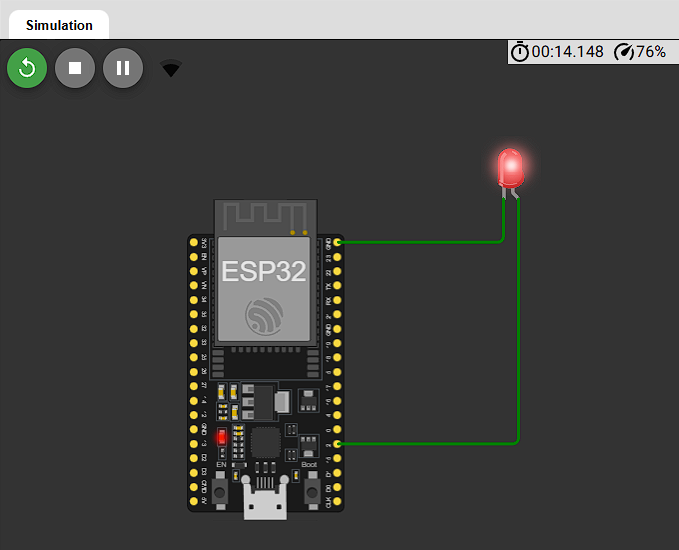
\includegraphics[width=0.7\textwidth]{../A15/wokwi.png}
    \caption{Simulation Wokwi - Atelier 15}
\end{figure}

\begin{figure}[H]
    \centering
    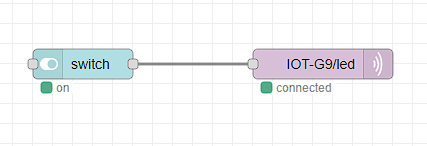
\includegraphics[width=0.6\textwidth]{../A15/flows.png}
    \caption{Flux Node-RED - Atelier 15}
\end{figure}

\begin{figure}[H]
    \centering
    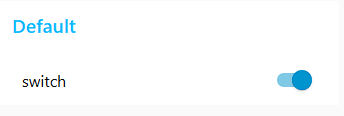
\includegraphics[width=0.6\textwidth]{../A15/dashboard.png}
    \caption{Dashboard - Atelier 15}
\end{figure}

\clearpage

\section*{Atelier 16 - Question 1 (A16-01)}

\textbf{Lien Wokwi :} \url{https://wokwi.com/projects/462396841658543105}

\vspace{0.3cm}
\textbf{Description :} Un système qui lit la température et l'humidité via un capteur DHT22 et les publie sur MQTT, tout en écoutant des commandes pour contrôler une LED. Les données sont visualisées sur un tableau de bord Node-RED (jauges) qui inclut un interrupteur pour la LED.
\vspace{0.5cm}

\begin{figure}[H]
    \centering
    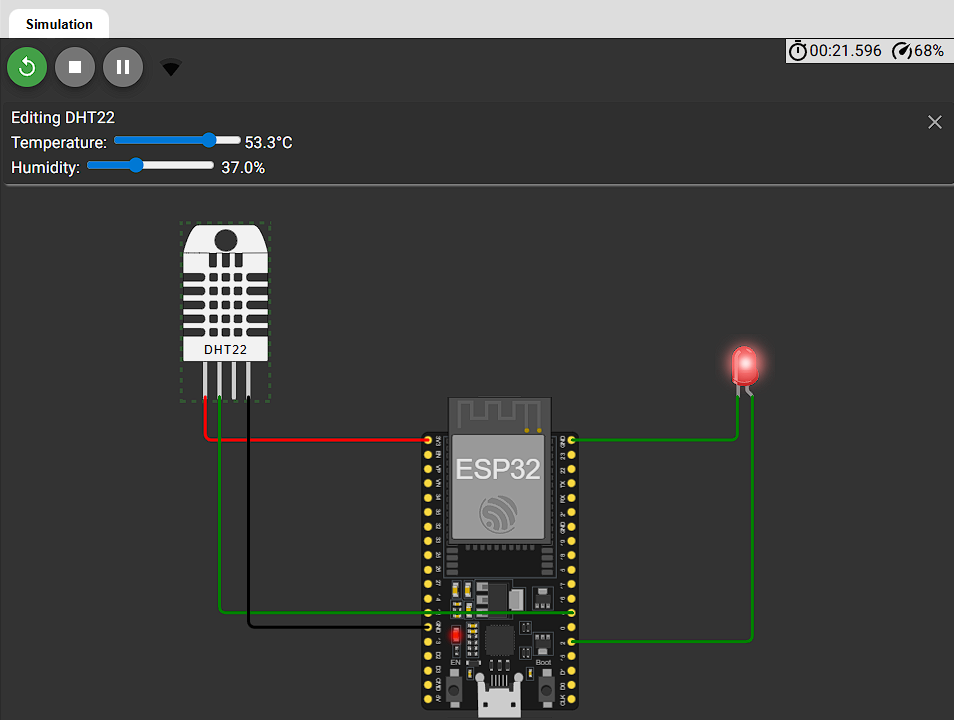
\includegraphics[width=0.7\textwidth]{../A16-01/wokwi.png}
    \caption{Simulation Wokwi - Atelier 16 Q1}
\end{figure}

\begin{figure}[H]
    \centering
    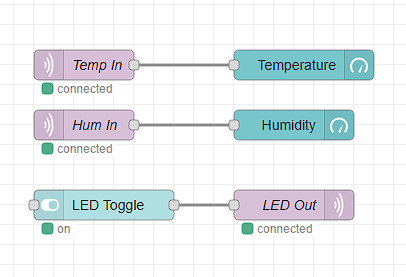
\includegraphics[width=0.7\textwidth]{../A16-01/flows.png}
    \caption{Flux Node-RED - Atelier 16 Q1}
\end{figure}

\begin{figure}[H]
    \centering
    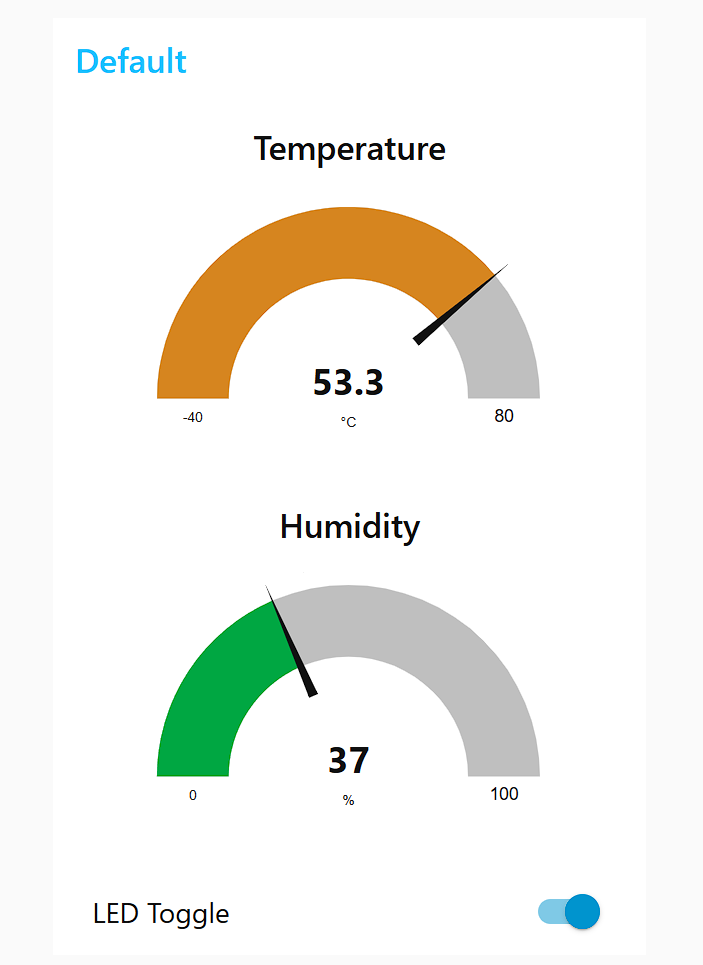
\includegraphics[width=0.7\textwidth]{../A16-01/dashboard.png}
    \caption{Dashboard - Atelier 16 Q1}
\end{figure}

\clearpage

\section*{Atelier 16 - Question 2 (A16-02)}

\textbf{Lien Wokwi :} \url{https://wokwi.com/projects/462399698002882561}

\vspace{0.3cm}
\textbf{Description :} Un système d'automatisation utilisant un servomoteur, un capteur de température (DHT22) et un capteur de luminosité (LDR). Géré par Node-RED, le système bascule entre un mode manuel (via un slider) et un mode automatique qui ouvre ou ferme le store en fonction de la chaleur et de la luminosité pour réguler la pièce.
\vspace{0.5cm}

\begin{figure}[H]
    \centering
    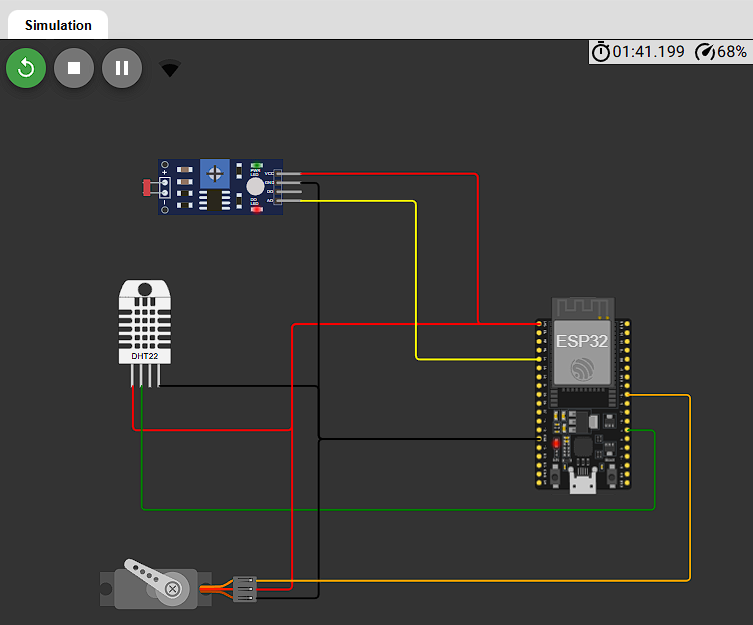
\includegraphics[width=0.7\textwidth]{../A16-02/wokwi.png}
    \caption{Simulation Wokwi - Atelier 16 Q2}
\end{figure}

\begin{figure}[H]
    \centering
    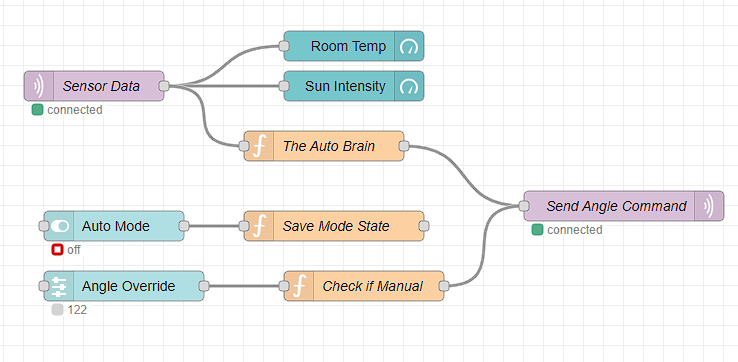
\includegraphics[width=0.7\textwidth]{../A16-02/flows.png}
    \caption{Flux Node-RED - Atelier 16 Q2}
\end{figure}

\begin{figure}[H]
    \centering
    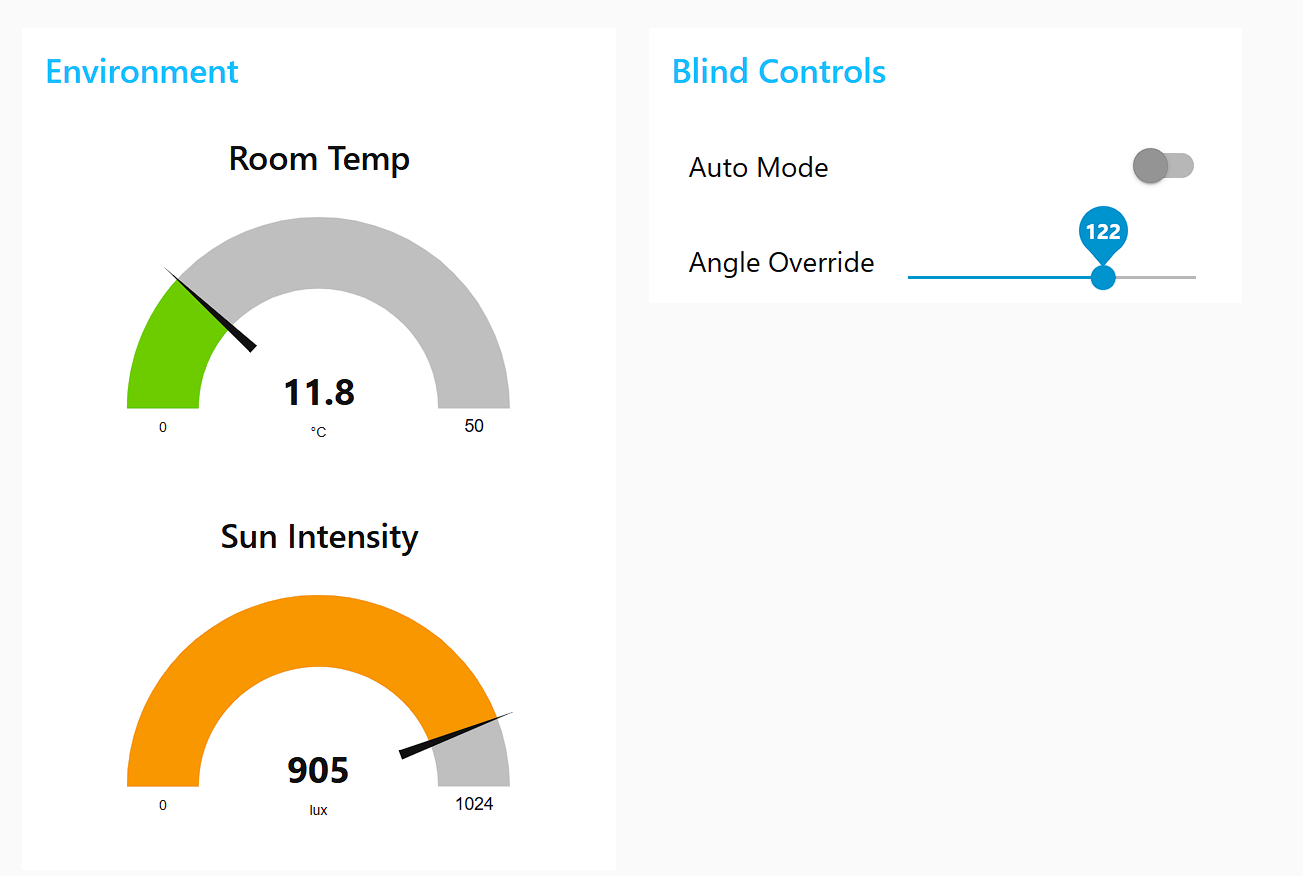
\includegraphics[width=0.7\textwidth]{../A16-02/dashboard.png}
    \caption{Dashboard - Atelier 16 Q2}
\end{figure}

\end{document}
